\documentclass[12pt, letterpaper, twoside]{article}
\usepackage[utf8]{inputenc}
 
\usepackage{listings}
\usepackage{color}
\usepackage{graphicx}
\usepackage{geometry}
 
 
\geometry{
 a4paper,
 left=10mm,
 top=20mm,
 }

\graphicspath{ {images/} } 
 
\definecolor{codegreen}{rgb}{0,0.6,0}
\definecolor{codegray}{rgb}{0.5,0.5,0.5}
\definecolor{codepurple}{rgb}{0.58,0,0.82}
\definecolor{backcolour}{rgb}{0.95,0.95,0.92}
 
\lstdefinestyle{mystyle}{
    backgroundcolor=\color{backcolour},   
    commentstyle=\color{codegreen},
    keywordstyle=\color{magenta},
    numberstyle=\tiny\color{codegray},
    stringstyle=\color{codepurple},
    basicstyle=\footnotesize,
    breakatwhitespace=false,         
    breaklines=true,                 
    captionpos=b,                    
    keepspaces=true,                 
    numbers=left,                    
    numbersep=5pt,                  
    showspaces=false,                
    showstringspaces=false,
    showtabs=false,                  
    tabsize=2
}
 
\lstset{style=mystyle}
 
 
 
\title{Numerical Methods for CSE}
\author{Nino Scherrer \thanks{based on NumCSE script from Prof. Dr. Hiptmaier}}
\date{FS2016}
 
\begin{document}
 
\begin{titlepage}
\maketitle
\end{titlepage}
 
 \section{General}

\subsection{Dense Matrix}

\subsection{Sparse Matrix}

“almost all” entries = 0 /“only a few percent of” entries $\not =$ 0"



\subsubsection{Build Matrix using Triples}

\begin{lstlisting}[language=C++, caption=Triplet example]

//Definition of a SparseMatrix
SparseMatrix<double> C(n,m);

//TripletList to save some triplets
std::vector<Triplet<double>> tripletList;

//Triplet entry
Triplet<double> triplet (i, j, value); 	 
//Saving Triplet in TripletList
tripletList.push_back(triplet);


//Fill Sparse Matrix with triplets in tripletList
C.setFromTriplets(tripletList.begin(), tripletList.end());
//Compress Sparse Matrix
C.makeCompressed();
	
\end{lstlisting}


\subsubsection{Special storage formats}
\paragraph{- COO (Triplet/Coordinate format)}
\paragraph{- CRS (Compressed row storage)}
\hspace{2mm}

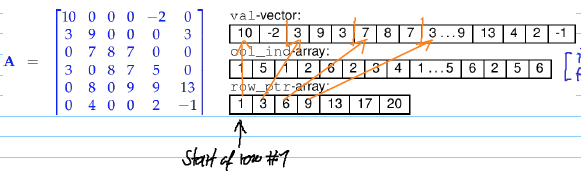
\includegraphics[width=0.8\textwidth]{SparseMatrix_CRS.png}








 
\end{document}